\documentclass{article}
\usepackage{graphicx} % Required for inserting images
\usepackage[utf8]{inputenc}
\usepackage[T1]{fontenc}
\usepackage{karnaugh-map}
\usepackage[polish]{babel}
\usepackage{subcaption}
\usepackage{float}
\usepackage{lmodern}
\usepackage{enumitem}
\usepackage{url}
\usepackage{array}
\usepackage{indentfirst}
\usepackage{amsmath}
\usepackage{booktabs}
\usepackage{caption}
\usepackage{hyperref}

\begin{document}
	
	\begin{center}
		% Używamy @{} aby usunąć zewnętrzne marginesy
		% Używamy 'm' (z pakietu 'array') dla środkowania w pionie
		
		\begin{tabular}{@{}|m{0.6\textwidth}|m{0.35\textwidth}|@{}}
			\hline
			% --- PIERWSZY WIERSZ LOGICZNY (wg obrazka) ---
			% Komórka 1,1 (Lewa-góra)
			Wydział Informatyki Politechniki Białostockiej \newline
			Przedmiot: Systemy operacyjne
			&
			% Komórka 1,2 (Prawa-góra)
			Data: 18.03.2026r. \\ \hline
			
			% --- DRUGI WIERSZ LOGICZNY (wg obrazka) ---
			% Komórka 2,1 (Lewa-środek)
			Temat: Projekt 1 – interfejs wywołań systemowych Linuksa. \newline
			
			& % <-- Separator kolumn dla wiersza 2
			
			% Komórka 2,2 (Prawa-środek)
			
			\\
			
			% --- TRZECI WIERSZ LOGICZNY (wg obrazka) ---
			% Komórka 3,1 (Lewa-dół)
			Grupa: PS8 \newline
			Imię i nazwisko: \newline
			Jakub Matusiewicz, Jakub Borkowski
			
			& % <-- Separator kolumn dla wiersza 3
			
			% Komórka 3,2 (Prawa-dół)
			Prowadzący: \newline
			mgr inż. Tomasz Kuczyński \\ \hline
		\end{tabular}
	\end{center}
	
	\section{Cel projektu}
	
	Celem projektu było stworzenie demona poszukującego plików, który w określonych odstępach czasu rekurencyjnie skanuje system plików w poszukiwaniu ścieżek dopasowanych do zadanych wzorców. Oprócz podstawowej funkcjonalności przeszukiwania i omijania plików bez uprawnień, celem było zaimplementowanie:
	\begin{itemize}
		\item \textbf{Współbieżności:} wykorzystania procesów potomnych (jeden proces roboczy na każdy podany argument) oraz procesu nadzorczego do zarządzania skanowaniem.
		\item \textbf{Komunikacji asynchronicznej:} obsługi sygnałów systemowych POSIX (\textbf{\texttt{SIGUSR1}}, \textbf{\texttt{SIGUSR2}}) do natychmiastowego wybudzania demona, restartowania lub przerywania trwającego przeszukiwania.
		\item \textbf{Szczegółowego raportowania:} zapisywania wyników wyszukiwania oraz opcjonalnych, wyczerpujących informacji o stanie procesu (tryb \textit{verbose}) do logu systemowego (\textbf{\texttt{syslog}}).
	\end{itemize}
	
	\section{Treść zadania}
	
	\textbf{Temat 2 - Demon(y) poszukujący plików}\\
	
	\textbf{[20p]} Demon(y) poszukujący plików. Program otrzymuje listę argumentów, z których każde jest fragmentem nazwy pliku. Program staje się demonem. Co kilkadziesiąt sekund (domyślny czas można zmienić za pomocą opcjonalnego parametru wiersza poleceń), rekurencyjnie skanuje system plików poszukując plików lub katalogów w których występuje zadany fragment nazwy. Pliki, do których demon nie ma praw dostępu są pomijane. Również takie katalogi są pomijane, dodatkowo katalog bez prawa odczytu i wykonania nie jest brany pod uwagę na etapie przeszukania rekurencyjnego. Nazwy odnalezionych plików lub katalogów są przekazywane zapisywane do logu systemowego (\textbf{\texttt{syslog}}). Umieszczone są w nim następujące informacje: pełna data, pełna ścieżka pliku, poszukiwany wzorzec. Odebranie sygnału \textbf{\texttt{SIGUSR1}} powoduje natychmiastowe rozpoczęcie skanowania, gdy demon śpi. Dodatkowa opcja \textbf{\texttt{-v}} powoduje przesyłanie do logu wyczerpującej informacji o każdej z następujących czynności demona: a) uśpienie, b) obudzenie się, c) odbiór sygnału, d) porównanie nazwy pliku ze ścieżką.\\
	
	\textbf{Dodatkowo:}
	\begin{enumerate}[label=\alph*)]
		\item \textbf{[6p]} Odebranie \textbf{\texttt{SIGUSR1}}, w chwili gdy trwa przeszukanie powoduje natychmiastowy restart przeszukiwania. Odebranie \textbf{\texttt{SIGUSR2}}, w chwili gdy trwa przeszukanie powoduje natychmiastowe zakończenie przeszukiwania i ponowne uśpienie demona.
		\item \textbf{[8p]} Przeszukanie jest prowadzone współbieżnie przez liczbę procesów równą liczbie argumentów. Dodatkowo występuje proces nadzorczy (śpi w oczekiwaniu na sygnały lub na zakończenie któregoś z procesów przeszukujących). Wysłanie procesowi nadzorczemu sygnału \textbf{\texttt{SIGUSR1}} albo \textbf{\texttt{SIGUSR2}} powoduje jego przekazania wszystkim procesom potomnym.
	\end{enumerate}
	
	\section{Opis poszczególnych modułów programu}
	
	Architektura projektu została podzielona na cztery główne, logiczne moduły funkcjonalne. Taki podział zapewnia czytelność i pozwala na separację mechanizmów systemowych (takich jak obsługa sygnałów i procesów) od logiki biznesowej (skanowanie plików).
	
	\subsection{Moduł Inicjalizacji, Konfiguracji i Głównej Pętli (\textbf{\texttt{main}}, \textbf{\texttt{args}}, \textbf{\texttt{daemonize}}, \textbf{\texttt{state}})}
	Moduł ten odpowiada za punkt wejścia do programu, wczytanie konfiguracji oraz transformację procesu w demona systemowego.
	\begin{itemize}
		\item \textbf{Opis działania:} Moduł parsuje argumenty z wiersza poleceń (\textbf{\texttt{args.c}}), w tym wzorce poszukiwań, opcjonalny czas uśpienia i flagę \textbf{\texttt{-v}} (verbose). Następnie wykonuje procedurę odpięcia programu od terminala (\textbf{\texttt{daemonize.c}}), powołując do życia demona. Proces demonizacji został dodatkowo zabezpieczony przed wielokrotnym niezamierzonym uruchomieniem za pomocą pliku PID z blokadą systemową (\textbf{\texttt{fcntl}} na \textbf{\texttt{/tmp/demonsearch.pid}}). W pliku \textbf{\texttt{state.h}} zdefiniowano współdzielone struktury konfiguracyjne i stałe czasowe (runtime), z których korzysta główna pętla w \textbf{\texttt{main.c}}.
		\item \textbf{Kluczowe zmienne globalne:} Struktura konfiguracyjna przechowująca listę argumentów (wzorców) do wyszukiwania, czas uśpienia oraz flagę trybu \textit{verbose}.
	\end{itemize}
	
	\subsection{Moduł Nadzorcy i Współbieżności (\textbf{\texttt{supervisor}}, \textbf{\texttt{proc\_table}}, \textbf{\texttt{worker}})}
	Moduł realizujący wymóg współbieżnego przeszukiwania na podstawie procesów potomnych oraz realizujący logikę procesu nadzorczego (supervisor).
	\begin{itemize}
		\item \textbf{Opis działania:} Plik \textbf{\texttt{supervisor.c}} implementuje orkiestrację procesu nadzorczego. Na podstawie ilości argumentów powoływane są procesy robocze (workery), realizowane w pliku \textbf{\texttt{worker.c}}. Każdy z nich odpowiada za jeden cykl skanowania dla przypisanego mu wzorca. Stan procesów (cykl życia, PID) jest rejestrowany i utrzymywany w strukturach modułu \textbf{\texttt{proc\_table.c}}, co ułatwia zarządzanie i ewentualne zabijanie/restartowanie workerów.
		\item \textbf{Kluczowe funkcje:} Funkcje monitorujące procesy potomne (\textbf{\texttt{wait}}/\textbf{\texttt{waitpid}}) oraz rozsyłające z procesu nadzorczego do workerów otrzymane sygnały (\textbf{\texttt{SIGUSR1}}/\textbf{\texttt{SIGUSR2}}).
	\end{itemize}
	
	\subsection{Moduł Skanowania Systemu Plików i Raportowania (\textbf{\texttt{scanner}}, \textbf{\texttt{match}}, \textbf{\texttt{logger}})}
	Moduł realizujący główną logikę operacji na plikach (I/O) i generowania logów.
	\begin{itemize}
		\item \textbf{Opis działania:} W module \textbf{\texttt{scanner.c}} zaimplementowano rekurencyjny bezpieczny traversal po systemie plików z uwzględnieniem sprawdzania praw dostępu do katalogów i plików. \textbf{\texttt{match.c}} służy jako moduł pomocniczy weryfikujący dopasowanie fragmentu nazwy pliku do zadanych wzorców z użyciem np. \textbf{\texttt{strstr}}. Architektura skanera została odseparowana od logiki raportowania przy użyciu mechanizmu wskaźników na funkcje (callbacks). Dzięki temu kod przechodzący po grafie katalogów operuje niezależnie od tego, co proces roboczy ostatecznie robi ze znalezioną ścieżką. Wyniki tych poszukiwań są ostatecznie wysyłane do systemowego logu przez specjalnie przygotowane funkcje z \textbf{\texttt{logger.c}}, które filtrują logi na standardowe oraz te dla opcji wyczerpującej (\textbf{\texttt{-v}}).
	\end{itemize}
	
	\subsection{Moduł Sygnałów i Usypiania (\textbf{\texttt{signals}}, \textbf{\texttt{sleep\_control}})}
	Moduł odpowiadający za komunikację asynchroniczną i sterowanie czasem wykonania programu za pomocą sygnałów POSIX.
	\begin{itemize}
		\item \textbf{Opis działania:} \textbf{\texttt{signals.c}} konfiguruje handlery dla sygnałów \textbf{\texttt{SIGUSR1}} (budzenie/restart skanowania) i \textbf{\texttt{SIGUSR2}} (przerwanie skanowania i uśpienie). Zmieniają one globalne flagi kontrolne. Z kolei \textbf{\texttt{sleep\_control.c}} używa tych flag do zarządzania interwałami snu nadzorcy i jego przedwczesnym wybudzaniem, wykorzystując bezpieczne dla systemu przerwania funkcji \textbf{\texttt{clock\_nanosleep()}}.
		\item \textbf{Kluczowe zmienne globalne:} Atomowe flagi systemowe (\textbf{\texttt{volatile sig\_atomic\_t}}), na których opiera się asynchroniczne przerywanie mechanizmu spania (obsługa błędu \textbf{\texttt{EINTR}}), powiadamiające demona, czy ma natychmiast przestać szukać czy zrestartować skanowanie.
	\end{itemize}
	
	\section{Zrzuty ekranu działającego programu (demonstracja)}
	
	W celu zaprezentowania poprawności działania programu, poniżej przedstawiono kilka kluczowych scenariuszy testowych, które zostały przeprowadzone na działającym demonie poszukującym plików. Każdy z nich ilustruje różne aspekty funkcjonalności, od standardowego działania po obsługę sygnałów i trybu verbose.

	\subsection{Walidacja argumentów i interfejs wiersza poleceń}
    Pierwszym etapem działania aplikacji jest parsowanie argumentów przekazanych przez użytkownika. Aby zapewnić stabilność demona i zapobiec nieprzewidzianemu zachowaniu systemu na skutek nieprawidłowych danych wejściowych, zaimplementowano rygorystyczny mechanizm weryfikacji. 

    Na Rysunku \ref*{fig:cli_args} zaprezentowano reakcję programu na niepoprawne wywołania. Aplikacja skutecznie wykrywa brak wymaganych wzorców wyszukiwania, brak wartości dla opcji wymagających parametru (np. czas interwału dla flagi \texttt{-i}), a także próby wielokrotnego zdefiniowania tej samej ścieżki (podwójna flaga \texttt{-d}). W każdym z tych przypadków program bezpiecznie przerywa działanie, wyświetlając komunikat błędu oraz wskazówkę dotyczącą użycia flagi pomocy (\texttt{-h}), która prezentuje pełną instrukcję obsługi.

    \begin{figure}[H]
        \centering
        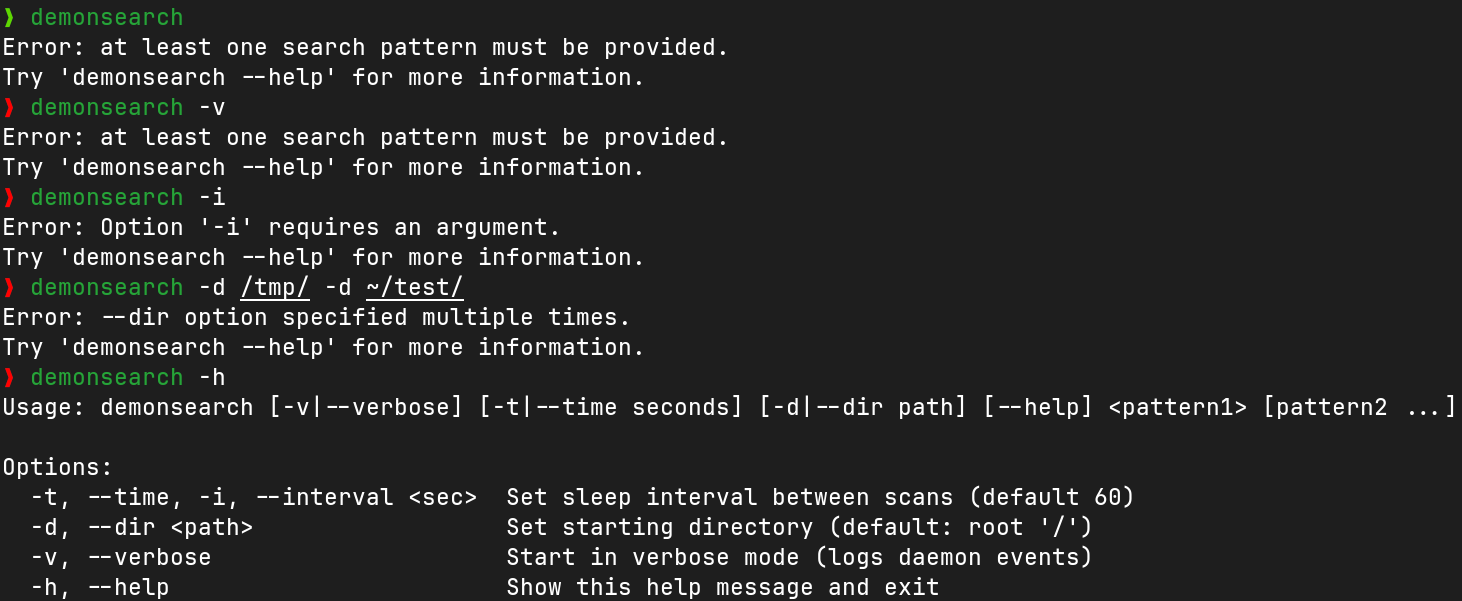
\includegraphics[width=\textwidth]{img0.png}
        \caption{Zrzut ekranu przedstawiający obsługę błędnych argumentów oraz pełny interfejs pomocy demona.}
        \label{fig:cli_args}
    \end{figure}
    
    \subsection{Standardowe uruchomienie z kilkoma wzorcami}
    Demon został wywołany z pięcioma poszukiwanymi wzorcami. Komenda \textbf{\texttt{ps u -C demonsearch}} (Rysunek \ref*{fig:ps}) potwierdza proces demonizacji i utworzenie dokładnie pięciu podprocesów powiązanych z procesem nadzorczym. Dodatkowo ujęto scenariusz pokazujący wysłanie sygnału zamknięcia (\texttt{kill}) do samego nadzorcy (supervisor), co skutkowało całkowitym wyczyszczeniem środowiska (\texttt{ps u} wykazał puste zwrócone linie), co dowodzi o bezpiecznym sprzątaniu i powiązaniu hierarchicznym procesów.
    
	\begin{figure}[H]
        \centering
        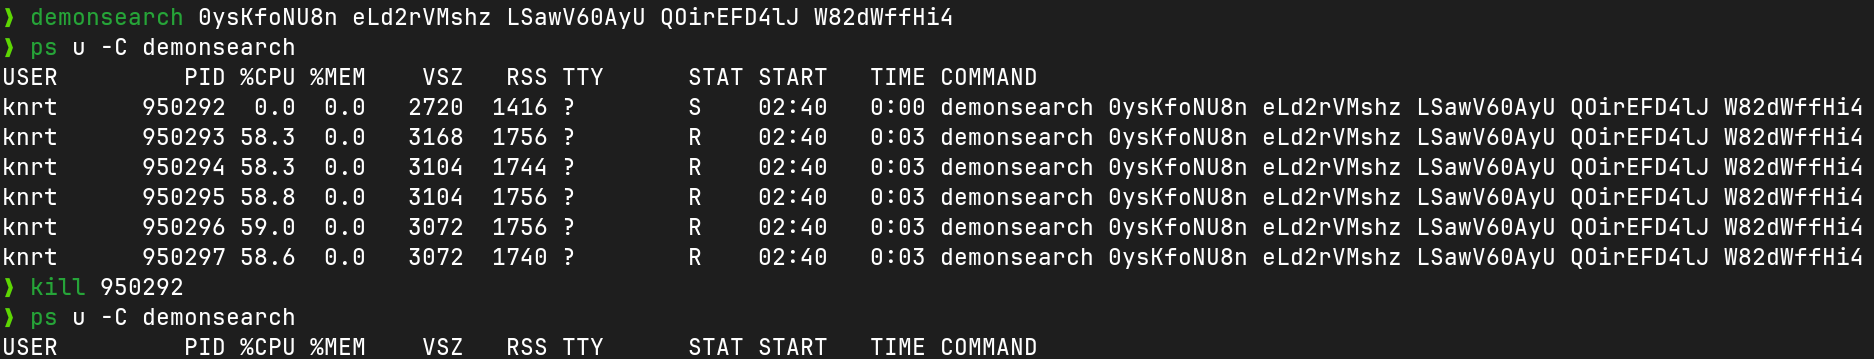
\includegraphics[width=\textwidth]{img1.png}
        \caption{Lista uruchomionych procesów demona oraz weryfikacja ich kaskadowego zamknięcia po uśmierceniu nadzorcy.}
        \label{fig:ps}
    \end{figure}
    
	Standardowe wyjście w systemowym dzienniku (Rysunek \ref*{fig:syslog}) potwierdza, że logowany jest czas, pełna ścieżka i powiązany z procesem na sztywno wzorzec (bez użycia PID'ów w treści, co eliminuje nieczytelność po restartach):
    
	\begin{figure}[H]
        \centering
        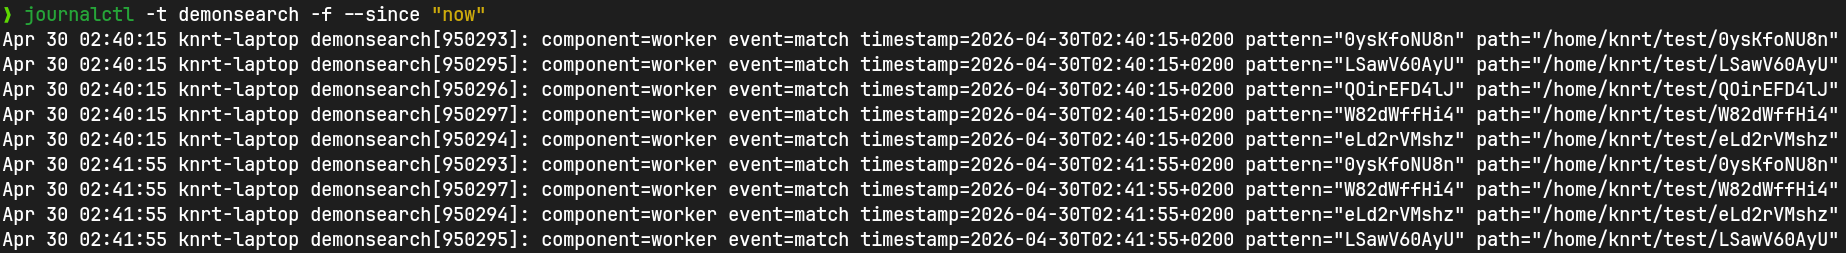
\includegraphics[width=\textwidth]{img2.png}
        \caption{Zrzut wpisów z dziennika po dopasowaniu plików do wzorców.}
        \label{fig:syslog}
    \end{figure}

\subsection{Szczegółowe monitorowanie skanowania z flagą -v (verbose)}
    Uruchomienie programu z opcją \texttt{-v} wymusza logowanie wyczerpujących informacji o każdym kroku wykonywanym przez demona, w tym o procesie analizy plików. Zrzut ekranu (Rysunek \ref*{fig:verbose_cmd}) ilustruje przykładowe polecenie testowe uruchamiające skanowanie wybranych wzorców z włączonym trybem \textit{verbose}.

    \begin{figure}[H]
        \centering
        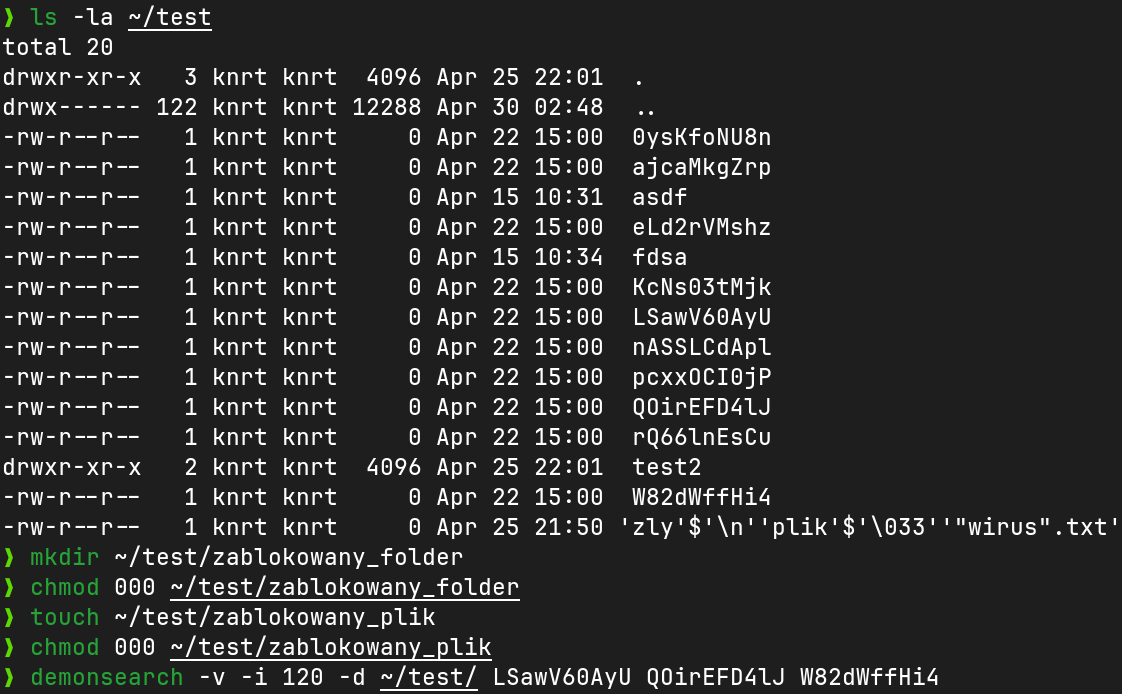
\includegraphics[width=\textwidth]{img3.png}
        \caption{Terminal pokazujący uruchomienie testowe programu demonsearch z włączoną flagą verbose.}
        \label{fig:verbose_cmd}
    \end{figure}

    Potwierdzeniem prawidłowego działania tego trybu są wpisy w dzienniku systemowym. Jak widać na Rysunku \ref*{fig:verbose_logs}, tryb \textit{verbose} generuje ogromną ilość logów dla zdarzenia skanowania. Widoczny jest moment startu procesu (event=\texttt{start}), rozpoczęcia przeszukiwania, a przede wszystkim logi typu \texttt{compare} informujące o ewaluacji każdej pojedynczej napotkanej ścieżki (z wynikiem \texttt{matched=true/false}). Dopiero po całkowitym przeanalizowaniu drzewa plików, worker loguje przejście w stan uśpienia (event=\texttt{state\_change}, state=\texttt{sleeping}).

    \begin{figure}[H]
        \centering
        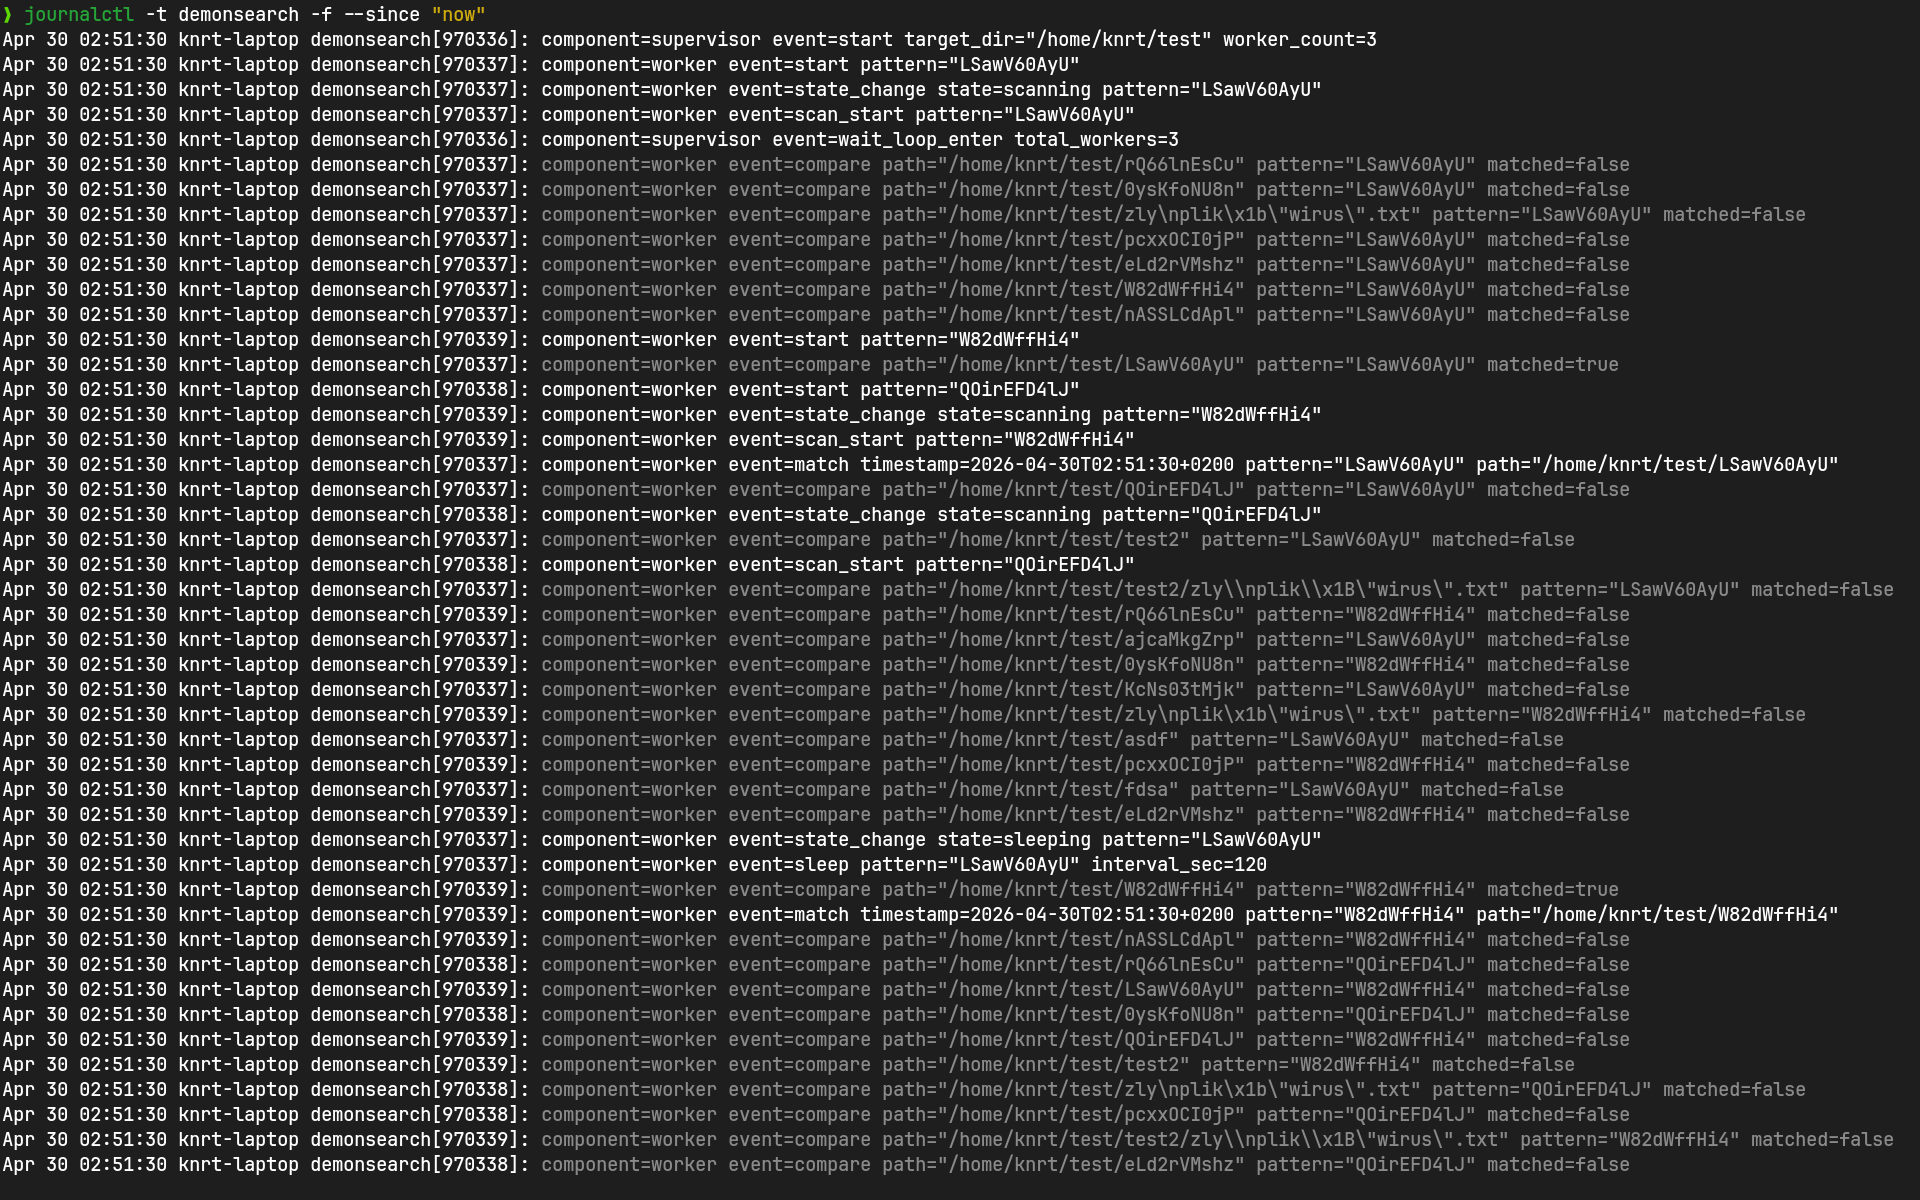
\includegraphics[width=\textwidth]{img4.png}
        \caption{Wyjście z logu systemowego demonstrujące wyczerpujące operacje workera (logi \texttt{compare}) wymuszone przez tryb verbose.}
        \label{fig:verbose_logs}
    \end{figure}

    \subsection{Wymuszone zatrzymanie pojedynczego procesu roboczego}
    Architektura demona zakłada niezależne i współbieżne działanie procesów potomnych. Aby zweryfikować poprawność zarządzania cyklem życia workerów oraz reakcję nadzorcy na niespodziewaną utratę procesu, przeprowadzono test polegający na ręcznym wysłaniu sygnału zakończenia do jednego z nich.\\[0.1cm]
    
    Na Rysunku \ref*{fig:kill_cmd} zaprezentowano stan procesów przed i po wykonaniu polecenia \texttt{kill}. Po wysłaniu domyślnego sygnału zamknięcia do wybranego workera (w tym przypadku PID 970338), znika on z listy aktywnych procesów, podczas gdy nadzorca i pozostałe procesy potomne nieprzerwanie kontynuują swoją pracę.

    \begin{figure}[H]
        \centering
        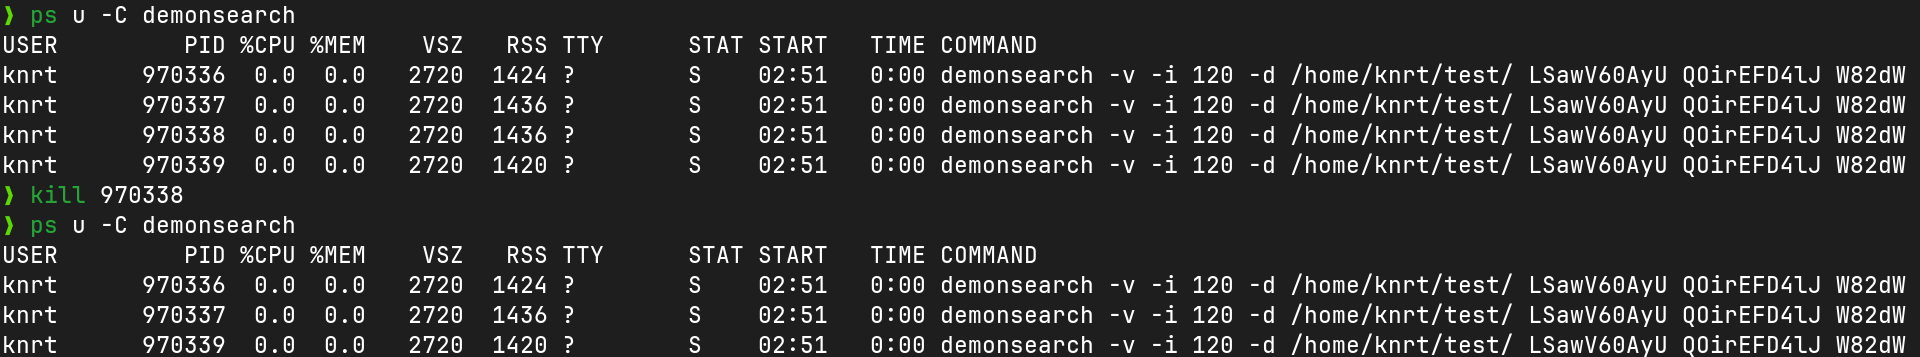
\includegraphics[width=\textwidth]{img5.png}
        \caption{Zrzut terminala ukazujący listę procesów demona przed i po ręcznym wyłączeniu pojedynczego workera.}
        \label{fig:kill_cmd}
    \end{figure}

    Faktyczną mechanikę tego zdarzenia można zaobserwować w logach aplikacji (Rysunek \ref*{fig:kill_log}). Wybrany worker przechwytuje sygnał 15 (\texttt{SIGTERM}) i wykonuje procedurę bezpiecznego wyłączenia, zwalniając przydzieloną pamięć (event=\texttt{shutdown}). Jednocześnie proces główny (nadzorca) natychmiast dowiaduje się o śmierci swojego potomka za sprawą sygnału 17 (\texttt{SIGCHLD}) wysłanego przez jądro systemu. Nadzorca prawidłowo obsługuje to przerwanie — aktualizuje swoją wewnętrzną tablicę procesów (\texttt{proc\_table}) i odnotowuje zaktualizowaną liczbę aktywnych workerów (\texttt{remaining\_workers=2}).

    \begin{figure}[H]
        \centering
        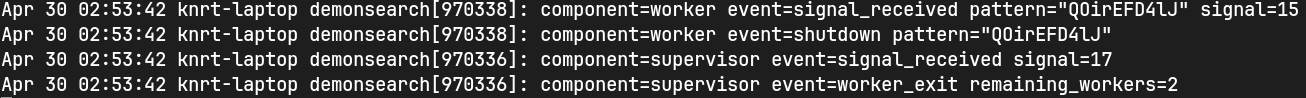
\includegraphics[width=\textwidth]{img6.png}
        \caption{Zapis z dziennika systemowego rejestrujący wymuszone zamknięcie workera (sygnał 15) oraz asynchroniczną reakcję nadzorcy (sygnał 17).}
        \label{fig:kill_log}
    \end{figure}

	\subsection{Asynchroniczna zmiana stanów i przerywanie skanowania (w locie)}
    Kolejnym testem weryfikującym poprawność wielobieżnej architektury demona było sprawdzenie jego reakcji na sekwencję sprzecznych poleceń. Celem było upewnienie się, że procesy robocze nie ignorują sygnałów, gdy są zajęte operacjami wejścia/wyjścia (I/O). Na Rysunku \ref*{fig:state_change_cmd} przedstawiono ciąg poleceń powłoki. Za pomocą narzędzia \texttt{pgrep} pobrano identyfikator nadzorcy, a następnie wysłano do niego w sekundowych odstępach sygnał uśpienia (12~--~\texttt{SIGUSR2}), sygnał wybudzenia/skanowania (10~--~\texttt{SIGUSR1}) oraz ponownie sygnał uśpienia (12). Test zakończono komendą \texttt{killall}.

    \begin{figure}[H]
        \centering
        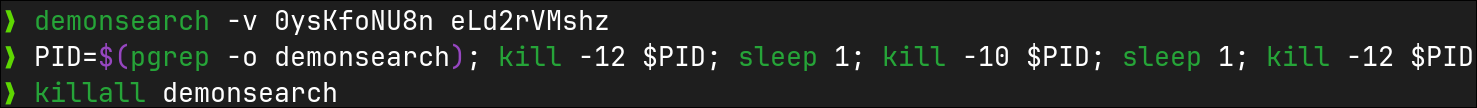
\includegraphics[width=\textwidth]{img7.png}
        \caption{Zrzut terminala z poleceniami wysyłającymi ręczną sekwencję sygnałów sterujących.}
        \label{fig:state_change_cmd}
    \end{figure}

    Analiza wygenerowanego dziennika (Rysunek \ref*{fig:state_change_log}) udowadnia poprawne działanie systemu. Nadzorca prawidłowo przekazał sygnały do workerów (event=\texttt{signal\_forward}). Kluczowym zachowaniem jest zarejestrowany wpis event=\texttt{scan\_interrupted}. Potwierdza on, że po wysłaniu sygnału \texttt{SIGUSR2} proces roboczy nie oczekiwał na całkowite zakończenie przeszukiwania dysku, lecz bezpiecznie je przerwał, przechodząc w stan uśpienia (event=\texttt{state\_change}, state=\texttt{sleeping}). Następujący bezpośrednio po nim sygnał wybudzenia prawidłowo wywołał zdarzenie \texttt{wakeup} i wznowił procedurę, po czym proces reagował na kolejne przerwania bez zawieszania się.

    \begin{figure}[H]
        \centering
        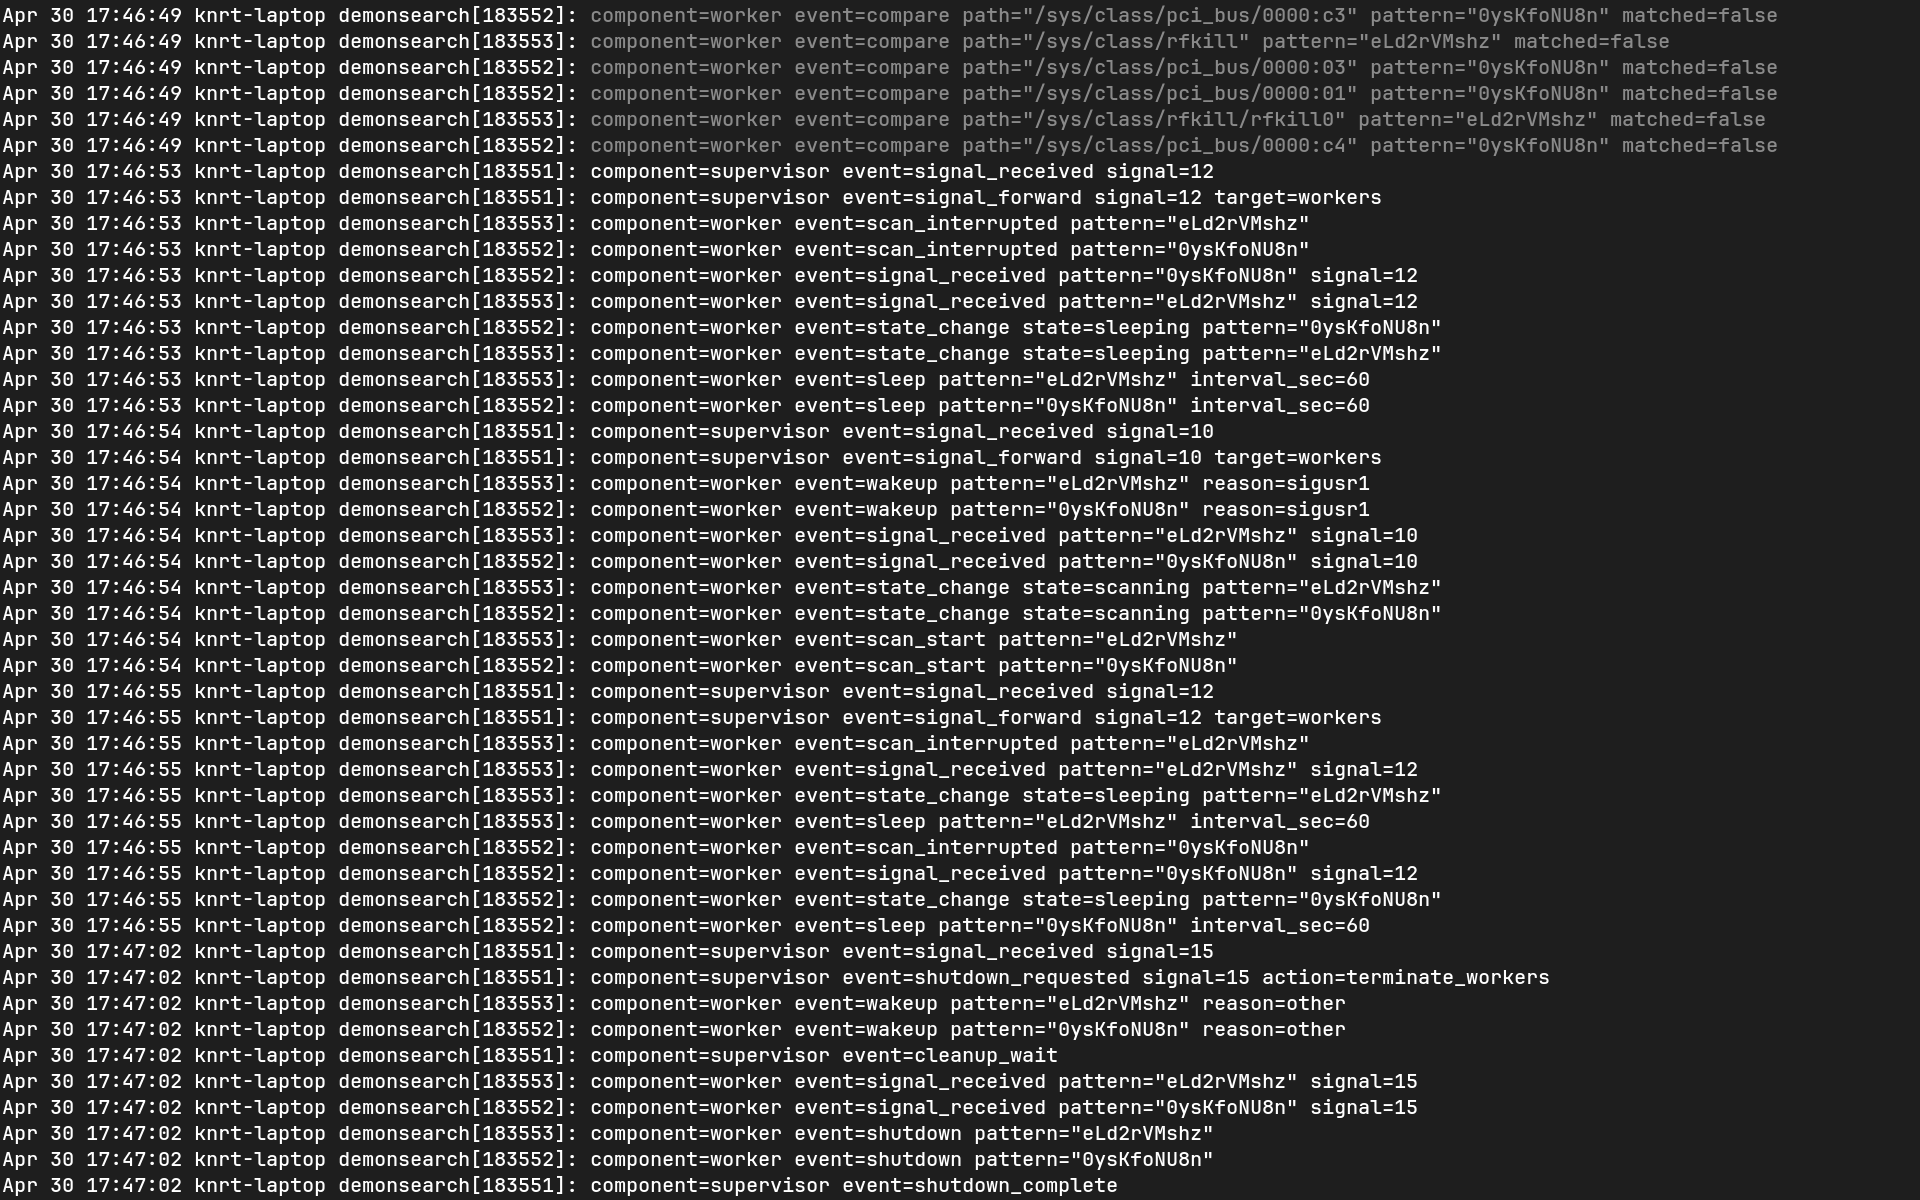
\includegraphics[width=\textwidth]{img8.png}
        \caption{Zapis dziennika pokazujący asynchroniczne przerywanie trwającego skanowania oraz płynne zmiany stanów wywołane poleceniami użytkownika.}
        \label{fig:state_change_log}
    \end{figure}

	\section{Podział pracy}
	\begin{itemize}
		\item \textbf{Jakub Borkowski:} Implementacja odpięcia procesu (\textbf{\texttt{daemonize}}), parsowania argumentów (\textbf{\texttt{args}}), procedury bezpiecznego i rekurencyjnego skanowania drzewa katalogów (\textbf{\texttt{scanner}}, \textbf{\texttt{match}}) oraz logowania do systemowego dziennika (\textbf{\texttt{logger}}).
		\item \textbf{Jakub Matusiewicz:} Pisanie sprawozdania, opracowanie obsługi sygnałów \textbf{\texttt{SIGUSR1}}/\textbf{\texttt{SIGUSR2}} i flag współdzielonych (\textbf{\texttt{signals}}), implementacja procesu nadzorczego i tabeli procesów do zarządzania potomkami (\textbf{\texttt{supervisor}}, \textbf{\texttt{proc\_table}}, \textbf{\texttt{worker}}) oraz kontrola wybudzania/usypiania głównej pętli (\textbf{\texttt{sleep\_control}}).
	\end{itemize}

\end{document}